% Created 2021-09-27 Mon 12:02
% Intended LaTeX compiler: xelatex
\documentclass[letterpaper]{article}
\usepackage{graphicx}
\usepackage{grffile}
\usepackage{longtable}
\usepackage{wrapfig}
\usepackage{rotating}
\usepackage[normalem]{ulem}
\usepackage{amsmath}
\usepackage{textcomp}
\usepackage{amssymb}
\usepackage{capt-of}
\usepackage{hyperref}
\setlength{\parindent}{0pt}
\usepackage[margin=1in]{geometry}
\usepackage{fontspec}
\usepackage{svg}
\usepackage{cancel}
\usepackage{indentfirst}
\setmainfont[ItalicFont = LiberationSans-Italic, BoldFont = LiberationSans-Bold, BoldItalicFont = LiberationSans-BoldItalic]{LiberationSans}
\newfontfamily\NHLight[ItalicFont = LiberationSansNarrow-Italic, BoldFont       = LiberationSansNarrow-Bold, BoldItalicFont = LiberationSansNarrow-BoldItalic]{LiberationSansNarrow}
\newcommand\textrmlf[1]{{\NHLight#1}}
\newcommand\textitlf[1]{{\NHLight\itshape#1}}
\let\textbflf\textrm
\newcommand\textulf[1]{{\NHLight\bfseries#1}}
\newcommand\textuitlf[1]{{\NHLight\bfseries\itshape#1}}
\usepackage{fancyhdr}
\pagestyle{fancy}
\usepackage{titlesec}
\usepackage{titling}
\makeatletter
\lhead{\textbf{\@title}}
\makeatother
\rhead{\textrmlf{Compiled} \today}
\lfoot{\theauthor\ \textbullet \ \textbf{2021-2022}}
\cfoot{}
\rfoot{\textrmlf{Page} \thepage}
\renewcommand{\tableofcontents}{}
\titleformat{\section} {\Large} {\textrmlf{\thesection} {|}} {0.3em} {\textbf}
\titleformat{\subsection} {\large} {\textrmlf{\thesubsection} {|}} {0.2em} {\textbf}
\titleformat{\subsubsection} {\large} {\textrmlf{\thesubsubsection} {|}} {0.1em} {\textbf}
\setlength{\parskip}{0.45em}
\renewcommand\maketitle{}
\author{Houjun Liu}
\date{\today}
\title{ISOS Day 1}
\hypersetup{
 pdfauthor={Houjun Liu},
 pdftitle={ISOS Day 1},
 pdfkeywords={},
 pdfsubject={},
 pdfcreator={Emacs 28.0.50 (Org mode 9.4.4)}, 
 pdflang={English}}
\begin{document}

\tableofcontents



\section{Epistomology}
\label{sec:org81f4810}
\textbf{Epistimology} => Episteme + Logos

\begin{quote}
Epistomology is the study of knowledge
\end{quote}

Epistomology: study of acquaintance

\section{Aftercare}
\label{sec:orgee6f056}
\subsection{The Semester}
\label{sec:orge44a0c5}
\begin{figure}[htbp]
\centering
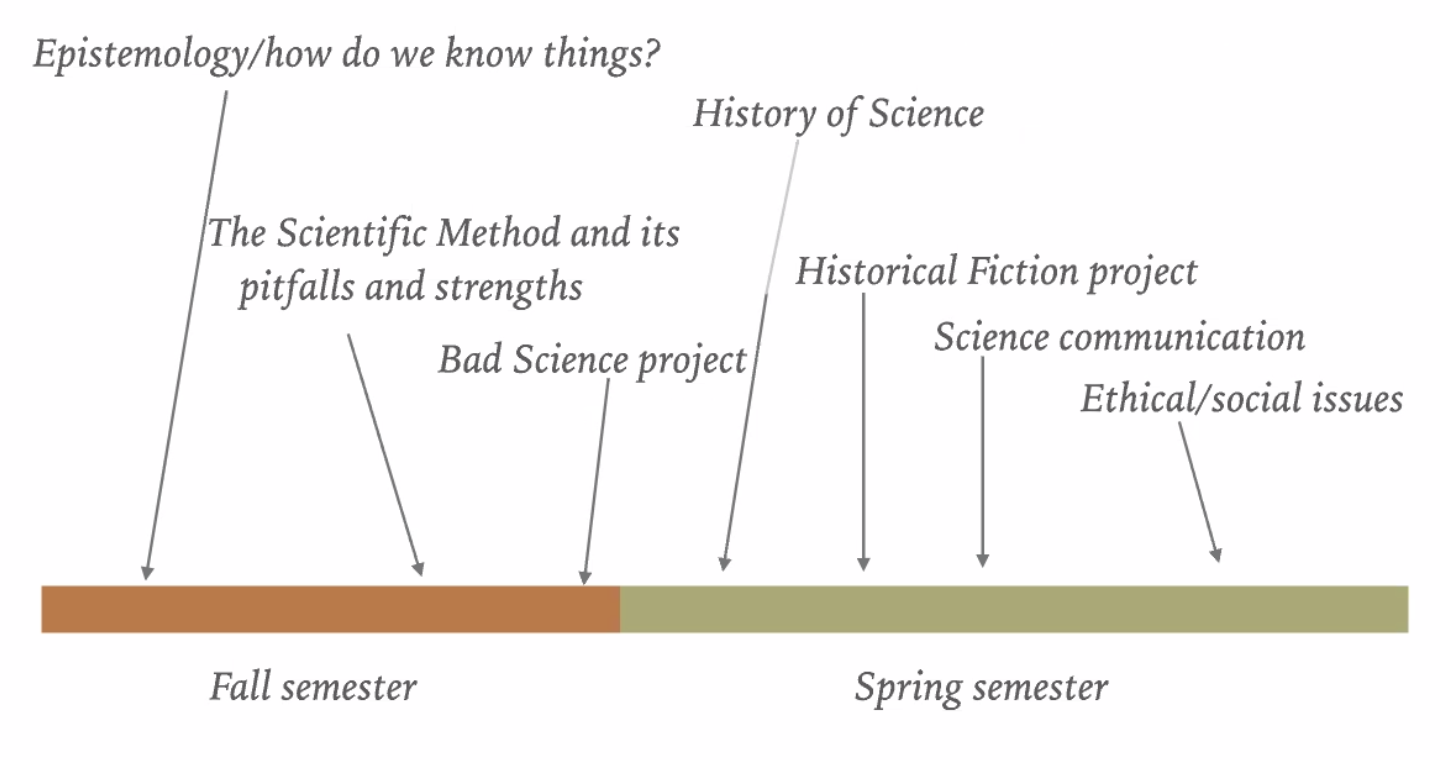
\includegraphics[width=.9\linewidth]{./2020ISOS101/Screen Shot 2020-08-25 at 2.23.23 PM.png}
\caption{Screen Shot 2020-08-25 at 2.23.23 PM.png}
\end{figure}

\subsection{FaQ}
\label{sec:orgf395490}
\begin{itemize}
\item How do I fail?

\begin{itemize}
\item Not doing the class
\end{itemize}

\item Is there a grade?

\begin{itemize}
\item No, the course is pass-fail
\end{itemize}

\item Can you fail?

\begin{itemize}
\item Yes
\end{itemize}

\item How to not fail?

\begin{itemize}
\item Do the class. Do the reading. Hand in assignments.
\end{itemize}

\item Homework?

\begin{itemize}
\item Yes, approx. 45 minutes/class. Reading + reflections => "Discussion
Points"
\end{itemize}
\end{itemize}

\section{Philosophy}
\label{sec:org0f8170c}
\emph{Plato}: Ideal Form \emph{Aristotle}: Down-to-Earthiness
\end{document}
